\section{Comportamento del Sistema}

\subsection{Descrizione del diagramma di sequenza} \label{SD-part1}

Nel seguente diagramma di sequenza è possibile vedere la rappresentazione dell'interazione tra attori tramite i messaggi descritti in precedenza.\newline

\begin{figure}[H]
	\begin{center}
		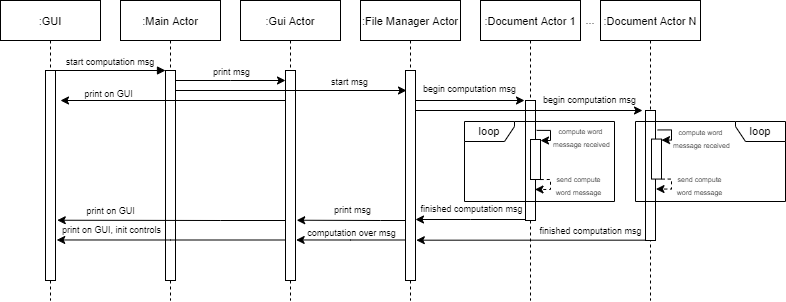
\includegraphics[width=1.1\linewidth]{img/part-1/document_actors_sequence.png}
		\label{fig:actors-seq-diagram}
	\end{center}
	\caption{Diagramma di sequenza del sistema}
\end{figure}

\subsection{Descrizione della Rete di Petri} \label{PN-part1}
% Descrizione del comportamento del sistema (ad un certo livello di astrazione)
% utilizzando Reti di Petri.
Il comportamento del sistema è stato modellato, ad un certo livello di astrazione, utilizzando una Rete di Petri.
\begin{question}[Rete di Petri]
Una Rete di Petri è un approccio grafico alla rappresentazione dei sistemi ad eventi in cui è possibile che alcuni eventi occorrano concorrentemente. Si tratta di un modello formale astratto del flusso di informazioni, descrive ed analizza il flusso di informazioni del sistema.
\end{question}

\noindent La seguente Rete di Petri descrive il flusso di informazioni del sistema ad attori proposto.\newline
Le piazze rappresentano gli attori creati e le transizioni sono i messaggi che vengono utilizzati per le comunicazioni tra attori.\newline

\begin{warn}[NOTA:]
Al fine di astrarre il funzionamento del sistema, si assume per semplicità di utilizzare 2 DocumentActors (ovvero 2 documenti da elaborare), uno costituito da 42 parole e l'altro da 13. Non è possibile specificare valori generici sul peso degli archi né un numero variabile di piazze, per cui non è possibile testare esaustivamente tutti gli scenari.
\end{warn}

\begin{figure}[H]
	\begin{center}
		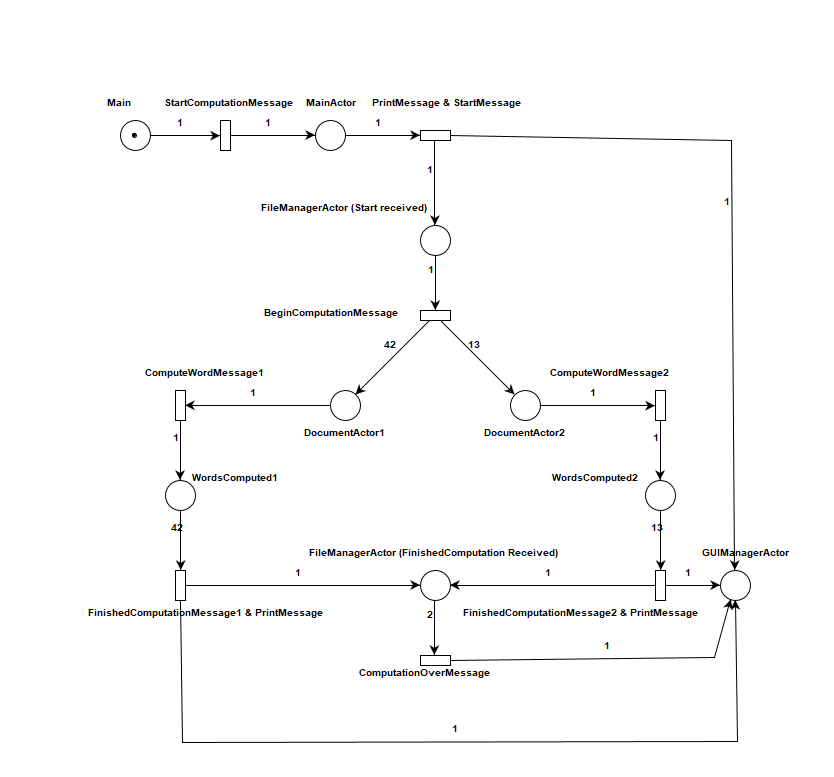
\includegraphics[width=\linewidth]{img/part-1/petri_net_actors.png}
		\label{fig:actors-petri-net}
	\end{center}
	\caption{Rete di Petri del sistema}
\end{figure}

\noindent La computazione inizia nella piazza Main, che passa il controllo alla piazza MainActor quando occorre iniziare la computazione. Il token nella piazza MainActor abilita una transizione che ha un duplice funzione: un token va nella piazza GUIManagerActor (la quale nel sistema si occupa di stampare una notifica di inizio computazione) e un token invece finisce nella piazza FileManagerActor.\newline

\noindent A questo punto, l'unica transizione abilitata è BeginComputationMessage; l'assunzione che si è costretti a fare è relativa al numero di documenti e di parole presenti in ogni documento, in quanto non è possibile creare un numero di piazze e token variabili. Nel nostro caso ci sono 2 documenti, uno di 42 parole e l'altro di 13. Chiaramente l'approccio è scalabile a un numero maggiore di documenti andando semplicemente ad aggiungere ulteriori piazze.\newline

\noindent La piazza DocumentActor1 è quindi stata popolata di \textit{42} token, i quali devono necessariamente essere tutti consumati per abilitare la transizione successiva. Tramite ComputeWordMessage viene consumato un token per volta, rappresentando la chiamata ricorsiva che il DocumentActor esegue per elaborare tutte le parole del documento.\newline
Quando la piazza WordComputed1 raggiunge il numero di token richiesto, la transizione abilitata genera un token nella piazza GUIManagerActor e nel FileManagerActor: quest'ultimo attende la fine dell'elaborazione di tutti i documenti prima di abilitare l'ultima transizione, che segnala il completamento totale della computazione.\newline

\noindent Il comportamento appena descritto per DocumentActor1 è del tutto analogo a DocumentActor2; ciò che è importante notare è che agiscono in modo del tutto autonomo e indipendente tra loro. L'ordine in cui vengono elaborate le parole e in cui i due attori terminano non è deterministico.
